\documentclass[class=book, crop=false, 11pt]{standalone}
\usepackage[subpreambles=true]{standalone}
\usepackage{import}
\usepackage[utf8]{inputenc}
\usepackage[margin=1.2in]{geometry}
\usepackage[sorting = none,
            doi = true  %lesedato for url-adresse
            ]{biblatex} %none gir bibliografi i sitert rekkefølge
\addbibresource{reference.bib}
\usepackage{csquotes}
\usepackage{amsmath}
\usepackage{amssymb}
\usepackage{makecell}


\usepackage{float}


\begin{document}
\chapter{Implementation}

This chapter will introduce the Python libraries \texttt{gym}, \texttt{stable-baselines} and \texttt{pandapower} that are used for setting up the reinforcement learning algorithm and solving the power flow equations. Also, the class \texttt{ActiveEnv} developed for this thesis is presented. 


\section{Pandapower}
The central goal in this thesis is to keep values for current and voltage in an electrical power system within safety margins. It is therefore necessary to have a way to solve the power flow equations \eqref{eq:theory:power_flow_equation} and use the results to see if safety margins are violated. The tool for solving the power flow equation in this thesis is the Python package \texttt{pandapower} \cite{pandapower}. They describe themselves in the following way:

\begin{displayquote}
"pandapower builds on the data analysis library pandas and the power system analysis toolbox PYPOWER to create an easy to use network calculation program aimed at automation of analysis and optimization in power systems. What started as a convenience wrapper around PYPOWER has evolved into a stand-alone power systems analysis toolbox with extensive power system model library, an improved power flow solver and many other power systems analysis functions." \cite{pandapower_website}
\end{displayquote}

Pandapower is a time independent simulation tool that finds steady state solutions to a power flow problem. The power consumption and production at nodes in the power system can easily be updated as desired, and the power flow calculation will give the resulting voltage and current magnitudes.

This section will describe the different electrical elements available in pandapower and how they are physically modelled. In addition, it is shown how to take actions in the power system using the API of pandapower. It should be noted that this thesis uses version 1.6.1 of pandapower, which has some differences compared to the 2.0.1 version available at the current time of writing. For instance, the base power unit in the 1.6.1 is kilowatts, while it for the 2.0.1 is megawatts.

\subsection*{Lines}
The method \texttt{pandapower.create\_line} can be used to create a line element that can be connected between two buses. Pandapower offers many standard types lines for both underground cables and overhead transmission lines. Alternatively a line with custom parameters for impedance, line length, line diameter etc. can be specified with the method \texttt{pandapower.create\_line\_from\_parameters}. The lines are modelled using the $\pi$-equivalent model, described in section \ref{section:pi_model}.

\subsection*{Generators}
Pandapower has two generator types. The first type is simply called generator and is modelled as a PV-bus. In other words, the active power production $P$ and voltage magnitude $|U|$ are known when solving the power flow equations. Generators can be created using the method \texttt{pandapower.create\_gen}, where nominal values for apparent power and voltage can be specified. The second type is the static generator, where the active power $P$ and reactive power $Q$ is specified (PQ-bus). Static generators are created using \texttt{pandapower.create\_sgen}. Pandapower models power from the consumer perspective, so negative values for active power $P$ and reactive power $Q$ correspond to generation of power.

\subsection*{Loads}
The load in pandapower is modelled as a PQ-bus, where active and reactive power are known. Loads are created using the method \texttt{pandapower.create\_load}. The loads can also be modelled with constant impedance $Z$, current $I$ and $P$. In other words, replacing reactive power with current and impedance.

\subsection*{Transformers}
Pandapower offers both two-winding and three-winding transformers that can be created from standard types using the \texttt{pandapower.create\_transformer} method, or from parameters using the method
\texttt{pandapower.create\_transformer\_from\_parameters}. The transformers can be modelled as a $\pi$-transformer or a $t$-transformer. The transformers can have settings for tap-position and phase-shifting of the voltage, which are a possible control variables for a reinforcement agent.  

\subsection*{Storage}
The method \texttt{pandapower.create\_storage} creates a storage element to a power net. The storage element is modelled as a PQ-node. Because simulations in pandapower is time-independent and only find steady state solution, it does not update the capacity of a storage during power flow calculations. Available energy in the storage element must therefore be updated manually according to some predefined timescale when several power flow calculations are performed.  


\subsection{Data structures in pandapower}

Pandapower stores information about elements in an electric transmission system in pandas DataFrames, which make it easy to inspect the numeric output of a power flow calculation. Figure \ref{fig:method:loading_example_net} shows a 4 bus case net and the components included in it. 

\begin{figure}[H]
    \center
    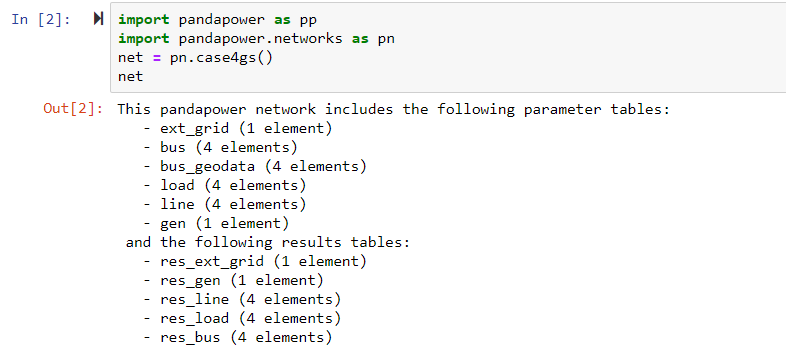
\includegraphics[height=6cm, width=12cm]{figures/case4g_show_net.PNG}
    \caption[size = 9]{Loading an example net in pandapower}
    \label{fig:method:loading_example_net}
\end{figure}
Each of the elements listed have a corresponding pandas DataFrame. The elements without "res" at the beginning are parameter tables and have information about nominal and max/min values for the components. Figure \ref{fig:method:line_bus_dataframe} shows the parameter table for the line and bus.

\begin{figure}[H]
    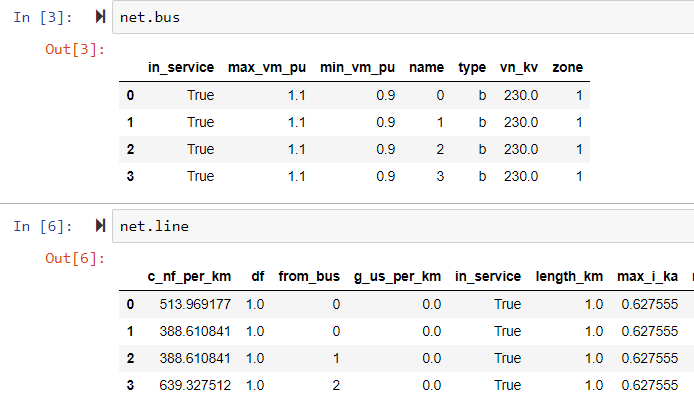
\includegraphics[height=8cm, width=13.5cm]{figures/case4g_line_bus.PNG}
    \caption[size = 9]{Parameter table in pandapower. There are more columns in \texttt{net.line}}
    \label{fig:method:line_bus_dataframe}
\end{figure}
All of the components will have a result table after the power flow calculation is performed, using the method \texttt{pandapower.runpp}. Figure \ref{fig:method:res_line_bus_dataframe} shows the result table for the bus and line. Note that values for active and reactive power are from the consumer perspective. In other words, positive values means consumption of power, while negative values means production.

\begin{figure}[H]
    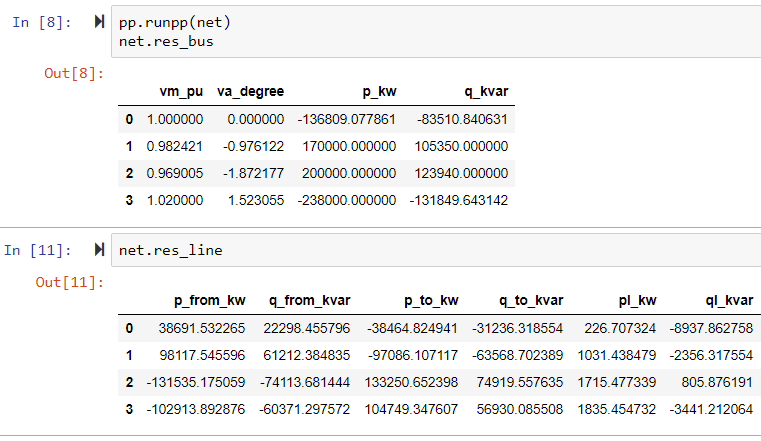
\includegraphics[height=8cm, width=14cm]{figures/case4g_line_bus_res.PNG}
    \caption[size = 9]{Result table in pandapower. There are more columns in \texttt{net.res\_line} than shown in the plot}
    \label{fig:method:res_line_bus_dataframe}
\end{figure}

\subsection{Plotting results}
It is important to be able to inspect the resulting state after a reinforcement agent performs an action on the system. This can be complicated for large network with many buses and lines that each have a voltage magnitude, voltage angle and so on. Fortunately, pandapower has support for plotting both grid architecture and results from the power flow. It is possible to get static plots using matplotlib and interactive plots using plotly \cite{plotly}. Figure \ref{fig:method:oberrhein_grid_results_plotly} shows the interactive results from a power flow calculation performed on the Oberrhein power grid using plotly. The lines are coloured based on the line loading (100\% means maximum current), while the buses are coloured based on the voltage magnitude. Such plots help to get an overview of the grid and quickly identify critical areas in the transmission system. It is possible to zoom into the net since the plot is interactive, and by clicking on a line or bus you can see the values for voltage, current and power.


\begin{figure}[H]
    \center
    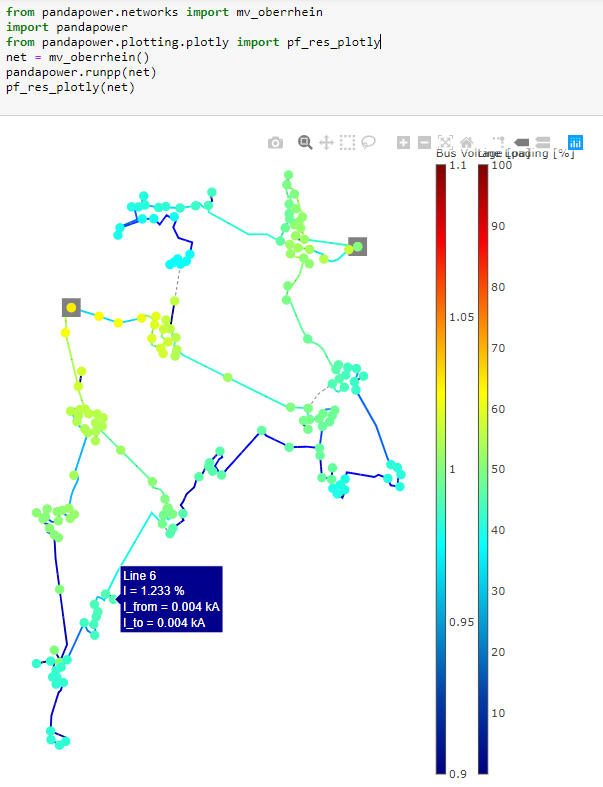
\includegraphics[height=15cm, width=12cm]{figures/results_pp_oberrhein.png}
    \caption[size = 9]{Interactive plot of the results from a power flow calculation on the Oberrhein case power grid using plotly. The grid consists of 179 lines and 180 buses}
    \label{fig:method:oberrhein_grid_results_plotly}
\end{figure}


\subsection{Controlling a pandapower net}
Reinforcement learning is all about taking actions and getting rewards based on how good that action was. It must therefore be possible to control certain elements in a pandapower net. This section will show how to perform certain actions in pandapower. \texttt{net.gen} gives a DataFrame where all the generators in the system is represented as a row. Because a generator is modelled as a PV-bus, it is possible to control the voltage and power by overwriting the parameters in \texttt{net.gen}. Figure \ref{fig:method:case4g_controll_vm_p_kw} shows how to set the active power production to 100000 kW and voltage magnitude to 0.99. The last row in the \texttt{net.res\_bus} is the bus where the generator is connected, and we see that the voltage magnitude is the same as the generator voltage magnitude. The power production if different from 100000 kW because there is a 80000 kW load connected to the same bus, and the table shows the sum of production and consumption at each bus. 



\begin{figure}[H]
    \center
    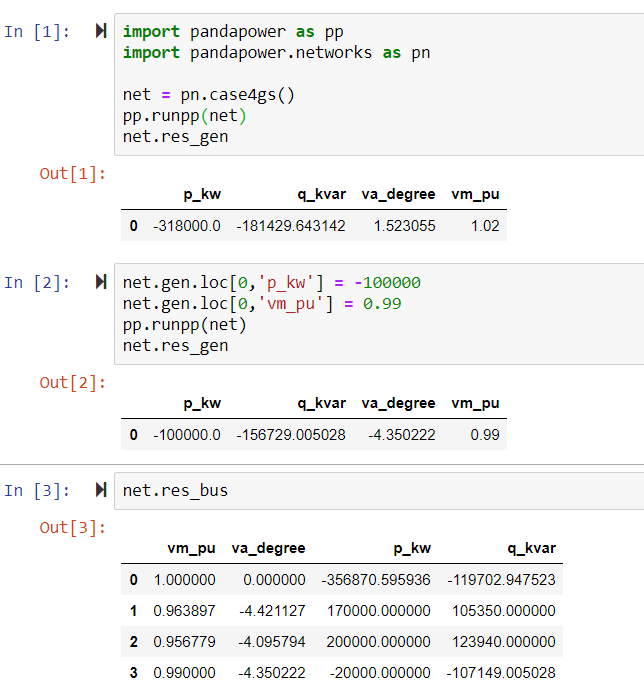
\includegraphics[height=12cm, width=12cm]{figures/case4g_controll_vm_p_kw.PNG}
    \caption[size = 9]{How to control the active power and voltage magnitude at a generator. Note that negative values for active power ('p\_kw') means production}
    \label{fig:method:case4g_controll_vm_p_kw}
\end{figure}

Transformers in a transmission system can have controllable taps that change the winding ratio between the low and high voltage side of the transformer. By doing this it is possible to control the voltage magnitude at buses connected to a transformer. There also exists phase-shifting transformers that can manipulate the the voltage angle between the low and high voltage side. Transformers in pandapower allow control of both voltage magnitude $|U|$ and voltage angle $\delta$. The code in figure \ref{fig:method:control_transformer} demonstrates how to control a transformer in pandapower. First, a two bus system with a transformer is created. It is a standard type transformer 25 MVA, 110/20 kV and the external grid is connected to the high voltage side of the transformer. The taps are placed on the low voltage side of the transformer with the command \texttt{net.trafo['tp\_side'] = 'lv'}. Performing a power flow calculation gives the result tables without changing the tap position in the transformer. The voltage angle is manipulated to 20 degrees by specifying \texttt{net.trafo['shift\_degree']}. The voltage magnitude is changed by first specifying \texttt{net.trafo['tp\_st\_percent']} which is the percentage change in voltage magnitude per tap position. This is set to 10 \% and the tap position is set using \texttt{net.trafo['tp\_pos']} to -1. By running another power flow calculation and inspecting the table \texttt{net.res\_bus}, it is evident that the voltage angle is shifted 20 degrees and that the voltage magnitude is reduced by 10 \% with respect to the first power flow calculation. 


\begin{figure}[H]
    \center
    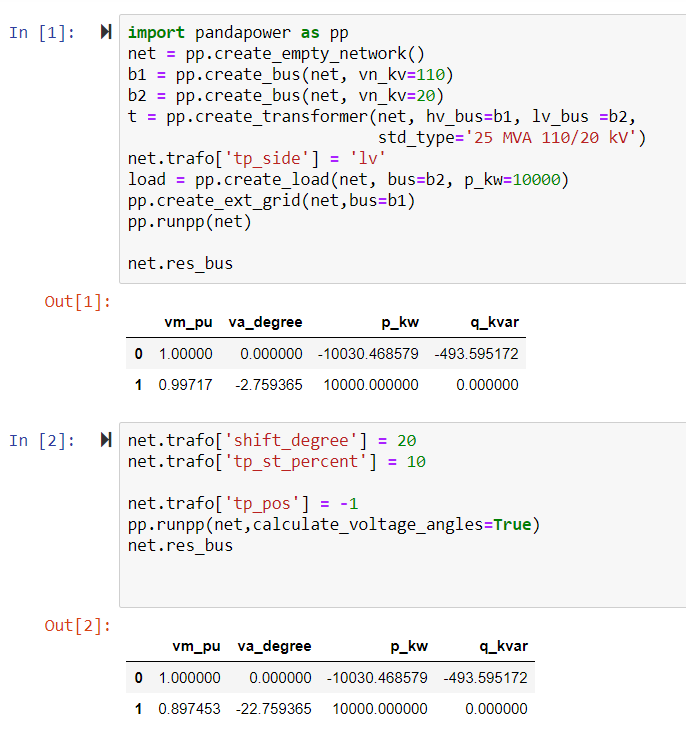
\includegraphics[height=12cm, width=12cm]{figures/control_transformer.PNG}
    \caption[size = 9]{Code showing how to control the tap position and phase angle for a transformer in pandapower}
    \label{fig:method:control_transformer}
\end{figure}

\section{Gym, stable-baselines and ActiveEnv}
The Python library \texttt{gym} is a toolkit used for managing environments in a reinforcement learning algorithm \cite{openai_gym}. It is developed by OpenAI and includes thousands of predefined environments of classical video games and control theory tasks such as the cartpole, swinging pendulum etc. In addition, it is possible to construct own environments that easily can be used in reinforcement algorithms. OpenAI also has a toolkit called \texttt{baselines} with implementations of many reinforcements algorithm that can interact with \texttt{gym} environments \cite{openai_baselines}. However, the \texttt{baselines} library is currently lacking a unified code structure between the algorithms and generally have poor documentation. As a result, a fork called \texttt{stable-baseline} has been created by the AI community, that offers a major cleanup of the code, with a scikit-learn like interface \cite{stable_baselines}. Along with this, it supports tensorboard that can be used to monitor the rewards and objective losses during training.

The implementation of the reinforcement algorithm in this thesis is done using \texttt{gym} and \texttt{stable-baselines}. Specifically, an environment class called \texttt{ActiveEnv} is implemented, that follows the standard \texttt{gym} environment structure. The main job \texttt{ActiveEnv} is to take in an action chosen by a reinforcement algorithm, perform that action, find the consequent state resulting from that action, and calculate the reward. Specifically, \texttt{ActiveEnv} receives an action vector $a$ where each component determines the percentage change in power consumption at each flexible load. First the consumption and production of power at nodes in the net are changed according to the demand forecast and solar forecast, respectively. The action vector is then processed and updates the power consumption at each load in the \texttt{pandapower} net. The power flow equations for the network are then solved using \texttt{pandapower}. Once the power flow equation have been solved and the new voltage and current magnitudes in the net are determined, the reward can be calculated. This summarises the steps involved with one action in the reinforcement algorithm. A more detailed description can be found in \ref{chap:problem_description}.   

There are many possible ways of constructing the reward function and state space, as discussed in \ref{chap:problem_description}. The \texttt{ActiveEnv} class has a method that can be used to specify the setup of the reinforcement learning algorithm, in addition to several parameters. Table \ref{table:implementation:param_description} gives a description of all the parameters together with their default values.  


{
\renewcommand{\arraystretch}{1.5}
\begin{table}[ht]
\center
\caption{Description of the parameters that determine the setup of the \texttt{ActiveEnv} environment}
\begin{tabular}{lll}
Parameter name     & Value                                                & Description                                                  \\
\hline
activation\_weight & 0.0001                                               & Weigh factor for activation cost                             \\
current\_weight    & 0.01                                                 & Weight factor for current cost                               \\
demand\_scale      & 10                                                   & Scale factor for power demand                                \\
demand\_std        & 0.03                                                 & \makecell[l]{Standard deviation as a ratio of \\ forecasted demand}           \\
episode\_length    & 200                                                  & \makecell[l]{Number of steps (hours) before the \\ environment resets}        \\
flexibility        & 0.1                                                  & \makecell[l]{Quantity describing  max demand change \\ at a load}              \\
forecast\_horizon  & 4                                                    & Number of hours in the forecasts                             \\
i\_upper           & 90                                                   & \makecell[l]{Upper current limit as percentage of \\line capacity}            \\
imbalance\_weight  & 0.0001                                               & Weight factor for imbalance cost                             \\
reactive\_power    & True                                                 & \makecell[l]{Determines if reactive power is \\ modified by the action}       \\
reward\_terms      & \makecell[l]{{[}’voltage’, ’current’,\\ ’imbalance’,’activation’{]}} & Terms to include in the reward function                      \\
solar\_scale       & 0.8                                                  & Scale factor for solar irradiance                            \\
solar\_std         & 0.03                                                 & \makecell[l]{Standard deviation as a ratio \\ of forecasted solar irradiance} \\
state\_space       & \makecell[l]{{[}’sun’, ’demand’, \\ ’imbalance’, 'bus'{]}}            & State spaces to be included in the model                     \\
total\_imbalance   & False                                                & \makecell[l]{Calculates total demand imbalance \\ in the system if True}      \\
v\_lower           & 0.95                                                 & Lower voltage margin                                         \\
v\_upper           & 1.05                                                 & Upper voltage margin                                         \\
voltage\_weight    & 1                                                    & Weight factor for voltage cost                              \\
\hline
\end{tabular}
\label{table:implementation:param_description}
\end{table}
}




\end{document}

